\documentclass[12pt]{article}

\usepackage{amsmath,amssymb}
\usepackage{graphicx}
\usepackage{subcaption}
\usepackage{booktabs}
\usepackage{siunitx}
\usepackage{mhchem}
\usepackage[
  backend=biber,
  style=authoryear,
  maxcitenames=2,
  mincitenames=1,
  uniquename=false,
  uniquelist=false
]{biblatex}
\addbibresource{refs/304IASCC.bib}
\graphicspath{{figures/}}

\DeclareSIUnit{\dpa}{dpa}
\DeclareSIUnit{\atpct}{at.\%}

% Same macros as main.tex
\newcommand{\Vac}{\mathrm{V}}
\newcommand{\Int}{\mathrm{I}}
\newcommand{\GB}{\mathrm{GB}}
\newcommand{\eff}{\mathrm{eff}}
\newcommand{\intf}{\mathrm{int}}
\newcommand{\thr}{\mathrm{th}}
\newcommand{\lat}{\mathrm{lat}}
\newcommand{\ox}{\mathrm{ox}}
\newcommand{\Ox}{\mathrm{O}}
% shorthands used in Sec. S3 (from notes/gb_channel_closure_derivation.tex)
\newcommand{\D}{D_{\Ox}^{\eff}}
\newcommand{\Cb}{\bar{C}_{\Ox}}
\newcommand{\Cc}{C_{\Ox}^{\mathrm{c}}}
\newcommand{\Ci}{C_{\Ox}^{\intf}}
\newcommand{\Jr}{J_{\mathrm{r}}}
\newcommand{\dd}{\mathrm{d}}

% Supplementary numbering
\renewcommand{\thesection}{S\arabic{section}}
\renewcommand{\thefigure}{S\arabic{figure}}
\renewcommand{\thetable}{S\arabic{table}}
\renewcommand{\theequation}{S\arabic{equation}}

\title{Supplementary Information\\[0.5em]
\large A Mechanistic Model for Radiation-Induced Segregation Controlled
Grain-Boundary Oxidation in Austenitic Stainless Steels}
\author{Zhuo Wang \and Md Shahrier Hasan \and Jaime Marian}
\date{\today}

\begin{document}
\maketitle

\section{Mesh Sensitivity of the Segregation Profiles and the Finite-Efficiency Sink Condition}
\label{sec:si-sink}

In an earlier version of the model the point-defect site fractions at the grain
boundary were fixed at their thermal-equilibrium values,
\begin{equation}
\left.C_{\Vac}\right|_{x=0}=C_{\Vac}^{\mathrm{eq}},\qquad
\left.C_{\Int}\right|_{x=0}=C_{\Int}^{\mathrm{eq}},
\label{eq:si-dirichlet}
\end{equation}
a Dirichlet condition that treats the boundary as a perfect sink. With this
condition the solution does not converge under mesh refinement. As the grid
spacing \(\Delta x\) is reduced, the point-defect profiles steepen at the
boundary, and both the gradient and the magnitude of the solute segregation
increase monotonically with refinement, Fig.~\ref{fig:si-mesh}(a--c). The width
of the segregation profiles likewise fails to converge. The same mesh
sensitivity has been reported for other Onsager-type RIS models
\parencite{oplinger2026radiationinduced}.

To remove this dependence the boundary is treated as a sink of finite
efficiency, i.e.\ a Robin condition on the defect fluxes,
\begin{align}
\left.\mathbf{J}_{\Vac}\!\cdot\!\hat{\mathbf{e}}_{x}\right|_{x=0}
 &= k_{\Vac}^{\GB}\left(\left.C_{\Vac}\right|_{x=0}-C_{\Vac}^{\mathrm{eq}}\right),
\label{eq:si-robin-vac}\\
\left.\mathbf{J}_{\Int}\!\cdot\!\hat{\mathbf{e}}_{x}\right|_{x=0}
 &= k_{\Int}^{\GB}\left(\left.C_{\Int}\right|_{x=0}-C_{\Int}^{\mathrm{eq}}\right),
\label{eq:si-robin-int}
\end{align}
where \(k_{\Vac}^{\GB}\) and \(k_{\Int}^{\GB}\) are the boundary transfer
coefficients of vacancies and self-interstitials and the flux is counted positive
towards the boundary. Equation~\eqref{eq:si-dirichlet} is the limit
\(k^{\GB}\to\infty\). With the Robin condition the profiles converge under
refinement, Fig.~\ref{fig:si-mesh}(d--f). The transfer coefficients
and the defect-mediated transport coefficients are calibrated jointly against the
magnitude and the width of the measured segregation profiles; the resulting
comparison at 0.5 and \SI{3.0}{\dpa} is shown in Fig.~2 of the main text.

\begin{figure}[!ht]\centering
\begin{subfigure}[t]{0.32\textwidth}\centering
  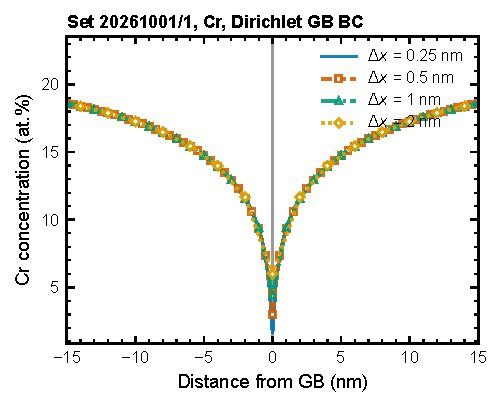
\includegraphics[width=\linewidth]{Cr_Dirich_vs_dx}
  \caption{}\label{fig:si-cr-dirich}
\end{subfigure}\hfill
\begin{subfigure}[t]{0.32\textwidth}\centering
  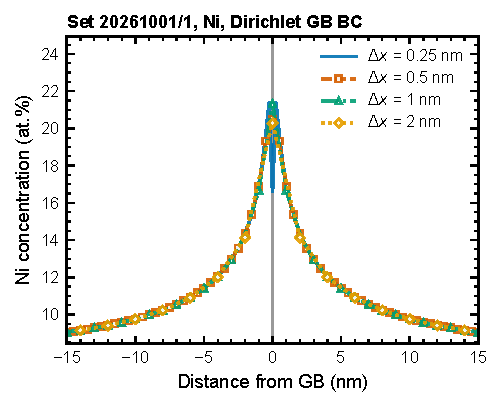
\includegraphics[width=\linewidth]{Ni_Dirich_vs_dx}
  \caption{}\label{fig:si-ni-dirich}
\end{subfigure}\hfill
\begin{subfigure}[t]{0.32\textwidth}\centering
  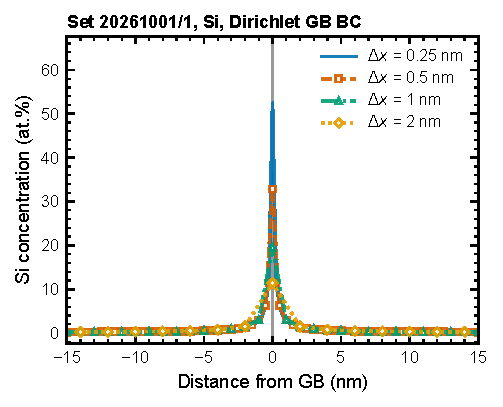
\includegraphics[width=\linewidth]{Si_Dirich_vs_dx}
  \caption{}\label{fig:si-si-dirich}
\end{subfigure}
\par\smallskip
\begin{subfigure}[t]{0.32\textwidth}\centering
  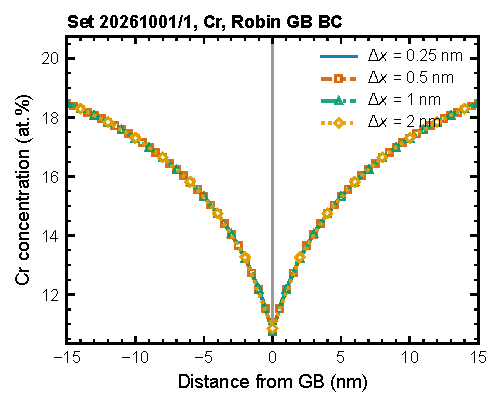
\includegraphics[width=\linewidth]{Cr_Robin_vs_dx}
  \caption{}\label{fig:si-cr-robin}
\end{subfigure}\hfill
\begin{subfigure}[t]{0.32\textwidth}\centering
  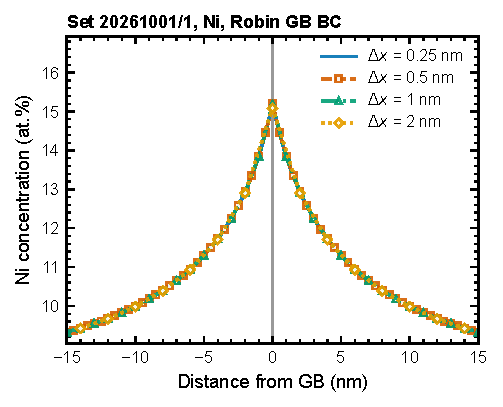
\includegraphics[width=\linewidth]{Ni_Robin_vs_dx}
  \caption{}\label{fig:si-ni-robin}
\end{subfigure}\hfill
\begin{subfigure}[t]{0.32\textwidth}\centering
  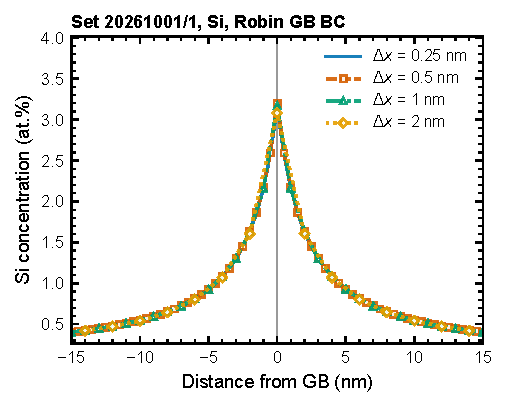
\includegraphics[width=\linewidth]{Si_Robin_vs_dx}
  \caption{}\label{fig:si-si-robin}
\end{subfigure}
\caption{Mesh sensitivity of the calculated Cr, Ni and Si concentration profiles
across the grain boundary for the two boundary conditions.
(a--c) Dirichlet (perfect-sink) condition, Eq.~\eqref{eq:si-dirichlet}, at grid
spacings \(\Delta x\) = 0.25, 0.5, 1 and \SI{2}{nm}. (d--f) Robin
(finite-efficiency) condition, Eqs.~\eqref{eq:si-robin-vac} and
\eqref{eq:si-robin-int}, at the same spacings.}
\label{fig:si-mesh}
\end{figure}

\section{Interfacial Mass Redistribution}
\label{sec:si-redistribution}

\subsection{Motivation}

In an earlier version of the model the metal removed at the oxidation front was
exactly the metal consumed by the four interfacial reactions, and all unoxidized
metal swept by the advancing front was rejected to the metal side of the
interface. Because the interfacial rate constant of Cr is much larger than that
of Fe, this assumption depletes Cr and enriches Fe strongly in the metal at the
interface. The EDX line scans of \textcite{deng2017effect} show the opposite
picture. The oxide is enriched in Cr and depleted in Fe, as expected for
selective oxidation, but the metal side of the interface shows no significant Cr
depletion or Fe enrichment, only a slight Ni enrichment. In the irradiated
specimens the Cr profile has a minimum at the centre of the oxide that deepens
with dose, which shows that the interfacial Cr concentration follows the
radiation-induced segregation profile as the front advances and is not modulated
by the selective oxidation. The excess Fe and Ni must therefore leave the
interface by a path other than rejection into the metal. \textcite{deng2020corrosion}
proposed that they diffuse along the oxide grain boundaries to the surface, where
Fe takes part in the formation of the outer oxide particles. A small amount of Ni
is detected in the intergranular oxide but no Ni oxide is observed
\parencite{deng2021grain}, so Ni is treated as unoxidized solute, part of which
remains in the oxide.

\subsection{Formulation}

Let \(J_{\mathrm{r}}^{i}\) be the rate at which element
\(i\in\{\mathrm{Cr},\mathrm{Fe},\mathrm{Ni},\mathrm{Si}\}\) is consumed by the
interfacial reactions through the stoichiometric sinks of the main text, with
\(J_{\mathrm{r}}^{\mathrm{Ni}}=0\), and \(C_i^{\GB}\) its concentration at the
interface. The element with the largest ratio of consumption to availability
sets the velocity at which the front must advance into the metal to be supplied,
\begin{equation}
v_{\lat}^{\ox,\max}=\max_{i}\frac{J_{\mathrm{r}}^{i}}{C_i^{\GB}} .
\label{eq:si-sweep}
\end{equation}
The front sweeps element \(i\) at the rate \(v_{\lat}^{\ox,\max}C_i^{\GB}\), of
which \(J_{\mathrm{r}}^{i}\) is oxidized. The remainder,
\begin{equation}
E_i=\max\!\left(v_{\lat}^{\ox,\max}C_i^{\GB}-J_{\mathrm{r}}^{i},\,0\right),
\label{eq:si-excess}
\end{equation}
is zero for the element that sets \(v_{\lat}^{\ox,\max}\) and equals the full
swept amount \(v_{\lat}^{\ox,\max}C_{\mathrm{Ni}}^{\GB}\) for Ni. The excess is
partitioned between rejection into the metal and removal through the oxide. The
partition is controlled by a redistribution velocity \(v_i^{\mathrm{r}}\) for
each element, the characteristic velocity at which element \(i\) can be rejected
into the metal ahead of the moving front. The fraction removed through the oxide
is
\begin{equation}
\lambda_i=\frac{v_{\lat}^{\ox,\max}}{v_{\lat}^{\ox,\max}+v_i^{\mathrm{r}}},
\label{eq:si-lambda}
\end{equation}
and the net removal of element \(i\) from the metal domain is
\begin{equation}
\tilde{J}_{\mathrm{r}}^{i}=J_{\mathrm{r}}^{i}+\lambda_i E_i .
\label{eq:si-sink}
\end{equation}
\(\tilde{J}_{\mathrm{r}}^{i}\) replaces \(J_{\mathrm{r}}^{i}\) as the outgoing
flux of element \(i\) at the boundary plane and in the recession rate of the
interface,
\begin{equation}
v_{\ox}=\sum_i\tilde{J}_{\mathrm{r}}^{i}
 =\sum_i J_{\mathrm{r}}^{i}+\sum_i\lambda_iE_i .
\label{eq:si-vox}
\end{equation}

\subsection{Limiting behaviour}

\begin{itemize}
  \item \(v_i^{\mathrm{r}}\to\infty\) for every element: \(\lambda_i=0\), the
        excess is rejected entirely into the metal, \(v_{\ox}=\sum_iJ_{\mathrm{r}}^{i}\),
        and the earlier formulation is recovered.
  \item \(v_i^{\mathrm{r}}\ll v_{\lat}^{\ox,\max}\) for every element:
        \(\lambda_i\to1\), the front outruns the rejection and the whole swept
        volume is removed. Since \(\sum_iC_i^{\GB}=1\),
        \(v_{\ox}=\sum_i v_{\lat}^{\ox,\max}C_i^{\GB}=v_{\lat}^{\ox,\max}\): the
        interface recedes at the sweep velocity, and the composition profile in
        the metal is translated rigidly without modification by the selective
        oxidation.
  \item Intermediate values give \(\sum_iJ_{\mathrm{r}}^{i}\le v_{\ox}\le v_{\lat}^{\ox,\max}\),
        with the partition set element by element.
\end{itemize}
The form of Eq.~\eqref{eq:si-lambda} is that of a solute-trapping law: the
fraction carried along by a moving interface is the ratio of the interface
velocity to the sum of the interface velocity and the velocity at which the
solute can escape ahead of it. The redistribution velocities are treated as
element-specific parameters; the element that sets \(v_{\lat}^{\ox,\max}\)
(Cr under the present conditions) has \(E_i=0\) and is unaffected by its value.

\subsection{Comparison with the line scans}

With the calculated oxide formed first placed at the centre of the intergranular
oxide, consistent with symmetric growth into both grains, the revised model
reproduces the central minimum of the Cr profile in the irradiated specimens and
its deepening with dose, together with the measured dose dependence of the Cr and
Fe contents of the oxide (Fig.~3 of the main text).

\section{Cross-Section-Averaged Oxygen Transport and the Lateral Closure}
\label{sec:si-closure}
\subsection{Purpose and result}

The grain-boundary oxidation model reduces oxygen transport to one dimension
along the boundary. This note treats the entire oxide cross-section as the
transport channel and derives, from the two-dimensional diffusion equation,
\begin{enumerate}
  \item[(i)] the one-dimensional balance for the cross-section-averaged oxygen
        concentration $\Cb$;
  \item[(ii)] a closure that gives the interfacial flux $\Jr$ directly from $\Cb$, the
        oxide half-width $L$, the diffusivity $\D$ and the interfacial reaction law
        $\Jr(\Ci)$.
\end{enumerate}
The closure is obtained from the separable solution of the Laplace equation in the
oxide cross-section. It reduces to one scalar equation for a dimensionless
eigenvalue $\mu\in(0,\pi/2)$,
\begin{equation}
\boxed{\;
\frac{\D\,\mu^{2}\,\Cb}{L}
 =\sum_k \Jr^{k}\!\bigl(\Cb\,\mu\cot\mu\bigr)
\;}
\label{eq:mu-eq}
\end{equation}
after which
\begin{equation}
\boxed{\;
\Jr=\frac{\D\,\mu^{2}\,\Cb}{L},
\qquad
\Ci=\Cb\,\mu\cot\mu
\;}
\label{eq:result}
\end{equation}
Equation~\eqref{eq:mu-eq} has a unique root and is solved pointwise by Newton's method,
in the same way as the series-resistance closure of the earlier model was solved for $\Ci$.

\subsection{Geometry and notation}
\label{sec:notation}

\begin{itemize}
  \item $y$: coordinate along the grain boundary, $y=0$ at the surface.
  \item $x$: coordinate normal to the boundary, $x=0$ on the boundary mid-plane
        (plane of symmetry). Only the half-domain $0\le x\le L$ is considered.
  \item $L(y,t)$: distance from the mid-plane to the oxide/metal interface. After the original boundary channel is filled.
  \item $C_{\Ox}(x,y,t)$: concentration of mobile (dissolved) oxygen in the oxide.
  \item $\D(y,t)$: effective oxygen diffusivity of the locally mixed oxide,
        Eq.~(15) of the main text. It is uniform across the section,
        because the phases are mixed locally rather than layered.
  \item Cross-section average, mid-plane value and interface value:
        \begin{equation}
        \Cb(y,t)=\frac{1}{L}\int_{0}^{L} C_{\Ox}\,\dd x,\qquad
        \Cc=C_{\Ox}(0,y,t),\qquad
        \Ci=C_{\Ox}(L,y,t).
        \end{equation}
  \item Interfacial oxygen flux (per unit boundary area, positive toward the metal):
        \begin{equation}
        \Jr(y,t)=-\D\,\frac{\partial C_{\Ox}}{\partial x}\bigg|_{x=L}.
        \label{eq:Jr-def}
        \end{equation}
  \item Interfacial reaction law: the total consumption
        $\Jr(\Ci)=\sum_k\Jr^{k}(\Ci)$ of
        the rate laws of the main text.
        It is a nondecreasing function of $\Ci$ at fixed metal concentrations. Where
        a linearized form is used below, $k\equiv\dd\Jr/\dd\Ci$.
\end{itemize}

\subsection{Assumptions}
\label{sec:assumptions}

\begin{enumerate}
  \item[A1.] Two-dimensional Fickian diffusion of oxygen in the oxide with a single,
        isotropic $\D$ that does not vary across the section.
  \item[A2.] Symmetry at the mid-plane: $\partial C_{\Ox}/\partial x=0$ at $x=0$.
  \item[A3.] Slow variation along the boundary of the half-width, the diffusivity and
        the metal concentrations that enter the reaction law:
        $|\partial L/\partial y|\ll1$, and $\D$, $\Jr(\cdot)$ change little over a
        distance $L$.
  \item[A4.] Lateral quasi-steady state: the lateral profile adjusts on the time scale
        $L^2/\D$, which is short compared with the time scales on which $\Cb$ and $L$
        change.
  \item[A5.] Locally, the lateral profile is the fundamental separable mode of the
        Laplace equation (Sec.~\ref{sec:mode}). Higher modes decay over a distance
        of order $0.3L$ or less and are neglected (Sec.~\ref{sec:validity}).
\end{enumerate}
No assumption is made on whether the interface is reaction- or diffusion-limited, and
no assumption is made that $C_{\Ox}$ is uniform across the section.

\subsection{Cross-section integration of the 2D balance}
\label{sec:integration}

The two-dimensional conservation equation in the oxide is
\begin{equation}
\frac{\partial C_{\Ox}}{\partial t}
 =\frac{\partial}{\partial y}\!\left(\D\,\frac{\partial C_{\Ox}}{\partial y}\right)
 +\D\,\frac{\partial^2 C_{\Ox}}{\partial x^2}.
\label{eq:2d}
\end{equation}
Integrate each term over $0\le x\le L(y,t)$, using the Leibniz rule where the limit
depends on $y$ or $t$.

\paragraph{Lateral term.} With A2 and the definition \eqref{eq:Jr-def},
\begin{equation}
\int_{0}^{L}\D\,\frac{\partial^2 C_{\Ox}}{\partial x^2}\,\dd x
 =\D\,\frac{\partial C_{\Ox}}{\partial x}\bigg|_{0}^{L}
 =-\Jr .
\label{eq:int-lateral}
\end{equation}

\paragraph{Time term.} Because the upper limit moves, the Leibniz rule gives the
identity
\begin{equation}
\frac{\partial}{\partial t}\int_{0}^{L}C_{\Ox}\,\dd x
 =\int_{0}^{L}\frac{\partial C_{\Ox}}{\partial t}\,\dd x
  +C_{\Ox}(L)\,\frac{\partial L}{\partial t},
\qquad\text{i.e.}\qquad
\int_{0}^{L}\frac{\partial C_{\Ox}}{\partial t}\,\dd x
 =\frac{\partial}{\partial t}\bigl(L\,\Cb\bigr)-\Ci\,\frac{\partial L}{\partial t}.
\label{eq:int-time}
\end{equation}
The last term is the dissolved oxygen, at concentration $\Ci$, contained in the
oxide formed during $\dd t$.

\paragraph{Along-boundary term.} Applying the Leibniz rule twice,
\begin{align}
\int_{0}^{L}\frac{\partial}{\partial y}\!\left(\D\frac{\partial C_{\Ox}}{\partial y}\right)\dd x
 &=\frac{\partial}{\partial y}\int_{0}^{L}\D\frac{\partial C_{\Ox}}{\partial y}\,\dd x
   -\D\,\frac{\partial C_{\Ox}}{\partial y}\bigg|_{x=L}\frac{\partial L}{\partial y},
\\
\int_{0}^{L}\D\frac{\partial C_{\Ox}}{\partial y}\,\dd x
 &=\D\left[\frac{\partial}{\partial y}\bigl(L\,\Cb\bigr)-\Ci\,\frac{\partial L}{\partial y}\right]
  =\D\,L\,\frac{\partial\Cb}{\partial y}
   +\D\,(\Cb-\Ci)\,\frac{\partial L}{\partial y}.
\end{align}
Hence
\begin{equation}
\int_{0}^{L}\frac{\partial}{\partial y}\!\left(\D\frac{\partial C_{\Ox}}{\partial y}\right)\dd x
 =\frac{\partial}{\partial y}\!\left(\D\,L\,\frac{\partial\Cb}{\partial y}\right)
  +\underbrace{\frac{\partial}{\partial y}\!\left[\D(\Cb-\Ci)\frac{\partial L}{\partial y}\right]
   -\D\frac{\partial C_{\Ox}}{\partial y}\bigg|_{x=L}\frac{\partial L}{\partial y}}_{O(\partial L/\partial y)} .
\label{eq:int-y}
\end{equation}

\paragraph{Result.} Collecting \eqref{eq:int-lateral}--\eqref{eq:int-y},
\begin{equation}
\frac{\partial}{\partial t}\bigl(L\,\Cb\bigr)
 =\frac{\partial}{\partial y}\!\left(\D\,L\,\frac{\partial\Cb}{\partial y}\right)
  -\Jr
  +\Ci\,\frac{\partial L}{\partial t}
  +O\!\left(\frac{\partial L}{\partial y}\right).
\label{eq:1d-exact}
\end{equation}
Equation~\eqref{eq:1d-exact} is exact. Under A3 the last group is dropped.

At the moving interface the diffusive flux $\Jr$ of \eqref{eq:Jr-def} supplies both
the reaction and the dissolved oxygen in the fresh oxide (Stefan condition, dissolved
oxygen in the metal neglected):
\begin{equation}
\Jr=\sum_k\Jr^{k}(\Ci)+\Ci\,\frac{\partial L}{\partial t}.
\label{eq:stefan}
\end{equation}
Substituting \eqref{eq:stefan} into \eqref{eq:1d-exact}, the terms
$\Ci\,\partial L/\partial t$ cancel and the sink is the reaction consumption alone.
The working one-dimensional equation is
\begin{equation}
\boxed{\;
\frac{\partial}{\partial t}\bigl(L\,\Cb\bigr)
 =\frac{\partial}{\partial y}\!\left(\D\,L\,\frac{\partial\Cb}{\partial y}\right)
  -\sum_k\Jr^{k}
\;}
\label{eq:1d-working}
\end{equation}
With $\partial L/\partial t=\Omega\sum_k\Jr^k$ and $\Omega=1/C_{\Ox}^{\mathrm{oxide}}$
the oxide volume formed per unit oxygen consumed, the ratio of the Stefan term in
\eqref{eq:stefan} to the reaction term is $\Ci/C_{\Ox}^{\mathrm{oxide}}\ll1$. The
diffusive flux $\Jr$ and the reaction consumption $\sum_k\Jr^k$ therefore differ by a
negligible amount, and from here on the single symbol $\Jr$ is used for both; in
particular the closure of Sec.~\ref{sec:mu} equates $\Jr$ of \eqref{eq:Jr-def} to
$\sum_k\Jr^k$.
Two remarks:
\begin{itemize}
  \item The along-boundary conductance is $\D L$ with the \emph{same} $\D$ as in the
        lateral direction. This follows from A1 alone; no assumption on the lateral
        profile was used.
  \item $L$ sits inside the time derivative. Expanding,
        $L\,\partial\Cb/\partial t=\partial_y(\D L\,\partial_y\Cb)-\Jr-\Cb\,\partial L/\partial t$;
        the last term is the dilution of dissolved oxygen as the section widens.
\end{itemize}
Equation~\eqref{eq:1d-working} contains two unknowns per position, $\Cb$ and $\Jr$.
The relation between them is derived next.

\subsection{Lateral problem: separation of variables}
\label{sec:mode}

\subsubsection{Local problem}

Under A3 and A4, in the neighbourhood of a given position along the boundary, the
oxide occupies a half-strip $0\le x\le L$ with $L$, $\D$ and the reaction law treated
as constants, and the concentration satisfies the steady equation
\begin{equation}
\frac{\partial^2 C_{\Ox}}{\partial x^2}+\frac{\partial^2 C_{\Ox}}{\partial y^2}=0,
\qquad
\frac{\partial C_{\Ox}}{\partial x}\bigg|_{x=0}=0,
\qquad
-\D\,\frac{\partial C_{\Ox}}{\partial x}\bigg|_{x=L}=\Jr\bigl(C_{\Ox}(L,y)\bigr).
\label{eq:laplace}
\end{equation}

\subsubsection{Separable solutions}

Seek $C_{\Ox}=X(x)\,Y(y)$. Substituting into the Laplace equation and dividing by
$XY$,
\begin{equation}
\frac{X''}{X}=-\frac{Y''}{Y}=-\left(\frac{\mu}{L}\right)^2,
\end{equation}
where the separation constant is written as $-(\mu/L)^2$ with $\mu>0$, because the
$x$-problem must be oscillatory (it has a homogeneous Neumann condition at $x=0$ and a
sink at $x=L$) and the $y$-dependence must decay into the boundary. Then
\begin{equation}
X''+\left(\frac{\mu}{L}\right)^2X=0,\quad X'(0)=0
\;\Rightarrow\;
X=\cos\!\left(\frac{\mu x}{L}\right);
\qquad
Y''-\left(\frac{\mu}{L}\right)^2Y=0,\;Y\to0
\;\Rightarrow\;
Y=e^{-\mu y/L}.
\end{equation}
Hence
\begin{equation}
C_{\Ox}(x,y)=A\,\cos\!\left(\frac{\mu x}{L}\right)e^{-\mu y/L},
\label{eq:mode}
\end{equation}
where $A$ is an amplitude and $\mu$ is to be fixed by the interfacial condition.
Different values of $\mu$ give different modes; the fundamental mode has the smallest
$\mu$ and the slowest decay in $y$, and by A5 it is the one retained.

\subsubsection{Averages and flux of the mode}

From \eqref{eq:mode}, with the common factor $e^{-\mu y/L}$ absorbed into $A$,
\begin{align}
\Cb&=\frac{A}{L}\int_{0}^{L}\cos\!\left(\frac{\mu x}{L}\right)\dd x
    =A\,\frac{\sin\mu}{\mu},
\label{eq:mode-avg}\\
\Ci&=A\cos\mu,
\label{eq:mode-int}\\
\Cc&=A,
\label{eq:mode-center}\\
\Jr&=-\D\,\frac{\partial C_{\Ox}}{\partial x}\bigg|_{x=L}
    =\frac{\D\,A\,\mu\sin\mu}{L}.
\label{eq:mode-flux}
\end{align}
Eliminating the amplitude with \eqref{eq:mode-avg}, $A=\mu\Cb/\sin\mu$, gives the
two relations of \eqref{eq:result}:
\begin{equation}
\Jr=\frac{\D\,\mu^{2}\,\Cb}{L},
\qquad
\Ci=\Cb\,\mu\cot\mu,
\qquad
\Cc=\frac{\mu\,\Cb}{\sin\mu}.
\label{eq:mode-relations}
\end{equation}
Both $\Jr$ and $\Ci$ are expressed through $\Cb$ and $\mu$ only. Note that
$\mu\cot\mu$ decreases monotonically from $1$ at $\mu=0$ to $0$ at $\mu=\pi/2$, so
$0\le\Ci\le\Cb$ for $\mu\in[0,\pi/2]$.

\subsubsection{Consistency with the averaged equation}

Substituting the mode into the steady form of \eqref{eq:1d-working} with constant
$L$ and $\D$,
\begin{equation}
\D L\,\frac{\partial^2\Cb}{\partial y^2}
 =\D L\left(\frac{\mu}{L}\right)^2\Cb
 =\frac{\D\,\mu^2\,\Cb}{L}
 =\Jr ,
\end{equation}
with no residual. The averaged equation and the mode closure are therefore mutually
consistent; no additional approximation is introduced by combining them.

\subsection{The equation for $\mu$}
\label{sec:mu}

\subsubsection{General (nonlinear) reaction law}

Imposing the interfacial condition of \eqref{eq:laplace} on the mode, and using
\eqref{eq:mode-relations} to express both sides through $\Cb$ and $\mu$,
\begin{equation}
g(\mu)\equiv\frac{\D\,\mu^{2}\,\Cb}{L}-\Jr\bigl(\Cb\,\mu\cot\mu\bigr)=0 .
\label{eq:g}
\end{equation}
This is Eq.~\eqref{eq:mu-eq}. It is a single scalar equation in $\mu$; the inputs are
the local values of $\Cb$, $L$, $\D$ and the metal concentrations that enter
$\Jr(\cdot)$.

\paragraph{Existence and uniqueness.} On $(0,\pi/2)$ the first term increases
monotonically from $0$; the second term decreases monotonically, because $\Jr(\cdot)$ is
nondecreasing and $\mu\cot\mu$ is decreasing. Hence $g$ is strictly increasing, with
\begin{equation}
g(0^+)=-\Jr(\Cb),
\qquad
g(\pi/2)=\frac{\pi^2\D\,\Cb}{4L}-\Jr(0).
\end{equation}
If $\Jr(\Cb)>0$ (oxidation possible at the local average concentration) and
$\Jr(0)\le0$ (no consumption at zero oxygen, which holds for all four rate laws,
including the magnetite law below its threshold), there is exactly one root
$\mu^\ast\in(0,\pi/2)$. If $\Jr(\Cb)\le0$, no oxygen is consumed: set $\mu=0$,
$\Jr=0$, $\Ci=\Cb$.

\paragraph{Newton iteration.} The derivative is
\begin{equation}
g'(\mu)=\frac{2\D\,\mu\,\Cb}{L}
        -\Jr'\bigl(\Ci\bigr)\,\Cb\,\frac{\dd}{\dd\mu}\bigl(\mu\cot\mu\bigr),
\qquad
\frac{\dd}{\dd\mu}\bigl(\mu\cot\mu\bigr)=\frac{\sin\mu\cos\mu-\mu}{\sin^2\mu}<0,
\end{equation}
so $g'>0$ throughout and Newton's method converges from any bracketed start. A
safeguarded Newton (fall back to bisection if an iterate leaves $(0,\pi/2)$) handles
the kink of the magnetite law at $\Ci=C_{\Ox}^{\mathrm{th}}$. A good initial guess is
the linearized value of Sec.~\ref{sec:linear}.

\paragraph{Algorithm per grid point and time step.}
\begin{enumerate}
  \item Inputs: $\Cb$, $L$, $\D$, $C_{\mathrm{Cr}}^{\GB}$, $C_{\mathrm{Fe}}^{\GB}$,
        $C_{\mathrm{Si}}^{\GB}$.
  \item If $\Jr(\Cb)\le0$: $\mu=0$, $\Jr=0$, $\Ci=\Cb$. Stop.
  \item Solve $g(\mu)=0$ on $(0,\pi/2)$ by safeguarded Newton.
  \item $\Jr=\D\mu^2\Cb/L$; $\Ci=\Cb\,\mu\cot\mu$; the individual $\Jr^{k}(\Ci)$
        give the metal sinks, the stoichiometric sinks of the main text, and the growth of each $L_k$.
  \item Use $\Jr$ as the sink in \eqref{eq:1d-working}.
\end{enumerate}
This replaces the series-resistance closure of the earlier model, which
also solves one scalar equation per point; the unknown is now $\mu$ instead of $\Ci$.

\subsubsection{Linearized reaction law}
\label{sec:linear}

For $\Jr=k\,\Ci$, Eq.~\eqref{eq:g} becomes
\begin{equation}
\frac{\D\mu^2}{L}=k\,\mu\cot\mu
\qquad\Longleftrightarrow\qquad
\mu\tan\mu=\frac{kL}{\D}\equiv\mathrm{Da},
\label{eq:mu-linear}
\end{equation}
the classical eigenvalue condition for a Robin boundary. $\mathrm{Da}$ is the ratio of
the lateral diffusion resistance $L/\D$ to the reaction resistance $1/k$. The
concentration $\Cb$ drops out: $\mu$ depends only on $\mathrm{Da}$.

\begin{table}[h]
\centering
\begin{tabular}{rrrr}
\toprule
$\mathrm{Da}=kL/\D$ & $\mu$ & $\Ci/\Cb=\mu\cot\mu$ & $\Jr L/(\D\Cb)=\mu^2$ \\
\midrule
$0$      & $0$     & $1$     & $0$ \\
$0.1$    & $0.311$ & $0.968$ & $0.097$ \\
$1$      & $0.860$ & $0.740$ & $0.740$ \\
$10$     & $1.429$ & $0.204$ & $2.042$ \\
$\infty$ & $\pi/2$ & $0$     & $\pi^2/4\approx2.467$ \\
\bottomrule
\end{tabular}
\caption{Fundamental mode for a linear reaction law.}
\label{tab:mu}
\end{table}

\subsubsection{Limits}

\begin{itemize}
  \item \textbf{Reaction-limited}, $\mathrm{Da}\ll1$: $\mu^2\simeq\mathrm{Da}$, so
        $\Jr\simeq k\,\Cb$ and $\Ci\simeq\Cb$. The interface sees the average
        concentration; the lateral profile is nearly uniform, with a parabolic
        deviation of relative size $O(\mathrm{Da})$. The decay length along the
        boundary is $L/\mu\simeq\sqrt{\D L/k}\gg L$.
  \item \textbf{Diffusion-limited}, $\mathrm{Da}\gg1$: $\mu\to\pi/2$, so
        $\Jr\to\pi^2\D\Cb/(4L)$ and $\Ci\to0$. Oxygen is consumed as soon as it
        reaches the interface; the lateral profile is a quarter cosine; the decay
        length along the boundary is $2L/\pi\approx0.64L$.
\end{itemize}
Between these limits $\mu$ interpolates smoothly. The closure never needs a
shape factor: if one insists on writing $\Jr=f\,\D(\Cb-\Ci)/L$, then
$f=\mu^2/(1-\mu\cot\mu)$, which runs from $3$ to $\pi^2/4$, but $f$ plays no role in
the algorithm.

\subsection{Range of validity}
\label{sec:validity}

\begin{enumerate}
  \item \textbf{Higher modes.} The interfacial condition admits a sequence of
        eigenvalues $\mu_0<\mu_1<\dots$, with $\mu_n\in(n\pi,\,n\pi+\pi/2)$ for a
        Robin condition. Each decays as $e^{-\mu_n y/L}$. The first higher mode decays
        at least as fast as $e^{-\pi y/L}$, i.e.\ over a distance $\lesssim L/\pi
        \approx0.3L$, compared with $\ge2L/\pi$ for the fundamental. Higher modes are
        excited where the boundary data change abruptly: the surface entry, the
        oxidation tip, and any position where $L$, $\D$ or the metal concentrations
        jump. Away from such places, only the fundamental survives (A5).
  \item \textbf{Slowly varying geometry (A3).} The mode is derived for a strip of
        constant width. For a wedge-shaped oxide the closure is applied with the local
        $L(y)$; the error is $O(\partial L/\partial y)$, the same order as the terms
        dropped in \eqref{eq:1d-exact}.
  \item \textbf{Quasi-steady lateral profile (A4).} Requires $L^2/\D$ to be short
        compared with the time scales of $\Cb(t)$ and $L(t)$. This can be checked
        from the simulation output.
  \item \textbf{Early stage.} When the oxidized zone is as deep as it is wide, the
        decay length is comparable to $L$ and the whole problem is two-dimensional.
        The one-dimensional description is meaningful only once the oxidized zone is
        slender; the initial aspect-ratio-one stage lies outside its scope.
  \item \textbf{Uniform $\D$ across the section (A1).} This is what allows the same
        $\D$ in \eqref{eq:1d-working} and \eqref{eq:laplace}. It follows from the
        local mixing of phases assumed in the main text.
\end{enumerate}

\subsection{Summary of the model change}
\label{sec:summary}

Earlier formulation:
\begin{align}
\frac{\partial C_{\Ox}}{\partial t}
 &=\frac{\partial}{\partial y}\!\left(\D\frac{\partial C_{\Ox}}{\partial y}\right)
   -\frac{\Jr}{\delta_{\GB}}, &
\Jr &=\D\,\frac{C_{\Ox}-\Ci}{\sum_k L_k}=\sum_k\Jr^{k}(\Ci).
\end{align}
Proposed formulation (cross-section average over the whole oxide, fundamental-mode
closure):
\begin{align}
\frac{\partial}{\partial t}\bigl(L\,\Cb\bigr)
 &=\frac{\partial}{\partial y}\!\left(\D\,L\,\frac{\partial\Cb}{\partial y}\right)-\Jr, &
\Jr &=\frac{\D\,\mu^{2}\,\Cb}{L},\quad
\frac{\D\,\mu^{2}\,\Cb}{L}=\sum_k\Jr^{k}\!\bigl(\Cb\,\mu\cot\mu\bigr).
\end{align}
What changes: (i) the storage width and along-boundary conductance are the
time-dependent half-width $L$ instead of the fixed $\delta_{\GB}$, with $L$ inside the
time derivative; (ii) the lateral closure is the fundamental Laplace mode, valid from
the reaction-limited to the diffusion-limited regime, with $\mu$ obtained pointwise
by Newton's method; (iii) $L$ is the mid-plane-to-interface distance. What does not
change: the reaction laws, the metal sinks, the definition of $\D$ as a local
volume-fraction average, and the structure of the pointwise scalar solve.

\section{Apparent Effective Diffusivities of the Oxidation Front}
\label{sec:si-deff}

Table~\ref{tab:si-deff} lists the apparent effective diffusivities
\(\bar{D}_{\mathrm{eff}}=L^{2}/2t\) computed from the reported final penetration
depth \(L\) and total exposure time \(t\) of the two experimental series used in
the main text. The values assume parabolic kinetics from \(t=0\) with no
incubation correction. At the same dose the oxide penetrates faster in the series
of \textcite{deng2020corrosion} than in that of \textcite{deng2017effect}; the
\SI{0.5}{\dpa} value of the former exceeds the \SI{3.0}{\dpa} value of the
latter. A model calibrated on the 2017 series is therefore expected to
underestimate the absolute depths of the 2020 series, as observed in Fig.~5 of
the main text. The normalized depth used there is
\begin{equation}
L_{\mathrm{norm}}=\frac{L}{L_{\max}},
\label{eq:si-lnorm}
\end{equation}
where \(L_{\max}\) is the maximum penetration depth over both doses, taken
separately for the calculations (\SI{110}{nm}) and for the measurements
(\SI{231}{nm}).

\begin{table}[htbp]
\centering
\caption{Apparent effective diffusivities of the grain-boundary oxidation
front, \(\bar{D}_{\mathrm{eff}}=L^{2}/2t\), from the reported final penetration
depth \(L\) and total exposure time \(t\). Depths for \textcite{deng2017effect}
are digitized from Fig.~12 therein (mean over the reported boundaries); depths
for \textcite{deng2020corrosion} are the values reported in the text.}
\label{tab:si-deff}
\begin{tabular}{llS[table-format=4.0]S[table-format=3.0]S[table-format=2.1]S[table-format=2.1]}
\toprule
Source & Dose & {\(t\) (\si{h})} & {\(L\) (\si{nm})} & {\(\bar{D}_{\mathrm{eff}}\) (\si{nm^2/h})} & {\(\bar{D}_{\mathrm{eff}}\) (\(10^{-22}\)~\si{m^2/s})} \\
\midrule
\textcite{deng2017effect}    & SA             & 500  & 40  & 1.6  & 4.4  \\
\textcite{deng2017effect}    & \SI{0.5}{\dpa} & 500  & 60  & 3.6  & 10.0 \\
\textcite{deng2017effect}    & \SI{3.0}{\dpa} & 500  & 100 & 10.0 & 27.8 \\
\textcite{deng2020corrosion} & \SI{0.5}{\dpa} & 1500 & 190 & 12.0 & 33.4 \\
\textcite{deng2020corrosion} & \SI{1.5}{\dpa} & 1500 & 240 & 19.2 & 53.3 \\
\bottomrule
\end{tabular}
\end{table}

\printbibliography

\end{document}
